\section{Common Hardware Implementation\label{sec:common_hardware_implementation}}

The four modules share a base hardware platform that is expanded upon to meet the requirements of the individual module. This section details the base platform and provides a rationale for it's implementation. It also details the process of schematic capture, board layout, and construction used for each module.

\nomenclature{PCB}{Printed Circuit Board}

\subsection{Base System Hardware\label{sec:base_system_hardware}}

All four modules are implemented on custom printed circuit boards (PCBs), and utilize a common base platform consisting of a \emph{micro-controller}, \emph{power supply}, \emph{status LEDs}, and a \emph{JTAG programming header}. The engine/transmission, braking, and telemetry modules also utilize a special sealed 23-pin \emph{connection header} to connect with the outside world. Table \ref{tab:common_module_components} lists the components in the common base package and their part numbers.

\begin{table}[H]
	\caption{List of hardware components common to each module.}
	\label{tab:common_module_components}
	\centering
	\begin{tabular}{|c|c|c|}
		\hline 
		Part & Manufacturer & Part Number \\ 
		\hline \hline
		Micro-Controller & Atmel & AT90CAN128 \\
		\hline
		Voltage Regulator & Linear Technology & LT1129CST5 \\
		\hline
		CAN Bus Transceiver & Microchip & MCP2551 \\
		\hline
		Connection Header & Tyco & AMPSEAL 1-770669-1 \\
		\hline
	\end{tabular}
\end{table}

\subsubsection{Micro-Controller}

Several low cost micro-controllers specifically designed for automotive use are available. Specifically, our design calls for a micro-controller with:

\begin{itemize}
  \item a \unit{5}{\volt} power supply;
  \item an integrated CAN bus controller;
  \item in-circuit debugging and programming capabilities; and
  \item a flexible cross-platform tool-chain.
\end{itemize}

\nomenclature{JTAG}{Joint Test and Action Group}

The 8-bit AT90CAN128 from Atmel meets all of these requirements, with the additional benefit of being platform we have developed for in the past. This micro-controller includes a \emph{Joint Test Action Group} (JTAG) standard debugging interface. Most importantly, there exists a well developed open-source tool-chain and standard ``C'' library.

\subsubsection{Voltage Regulator}

The LT1129 from Linear Technology was chosen as voltage regulator. This particular regulator is capable of supplying up to \unit{700}{\milli\ampere} of current. It requires only a single \unit{3.3}{\micro\farad} output capacitor, and accepts input voltages up to \unit{30}{\volt}. It also has built-in thermal limiting \cite{LTC1129}.

\subsubsection{CAN Bus Transceiver}

The modules communicate with each other over a two-wire CAN bus operating at 1 MBit/s. Each system module has a Microchip-brand MCP2551 CAN Transceiver IC to interface their local micro-controller to the bus. All modules are capable of being a termination point for the bus \cite{MCP2551}. 

\subsection{Schematic Capture and PCB Layout}

Schematic capture and PCB layout were both accomplished with CADSoft's ``Eagle''. All four modules are laid out on two-layer PCBs with a ground fill on the bottom and a \unit{+5}{\volt} fill on the top. This technique reduces the possibility of ground loops by making all ground connections as short as possible, and increases overall noise immunity. Fig.\ \ref{fig:driver_interface_layout} shows the telemetry module layout exported from Eagle. Both top and bottom conducting layers are indicated on the figure.

\subsection{Module Construction}

The printed circuit boards were manufactured by Alberta Printed Circuits (AP Circuits) Ltd., who kindly sponsored the project. Industry-standard GERBER-format files were generated from the PCB layouts and sent electronically to AP Circuits. Figure \ref{fig:empty_pcbs} shows a photograph of the four empty PCBs after they were manufactured.

\begin{figure}[H]
  \centering
  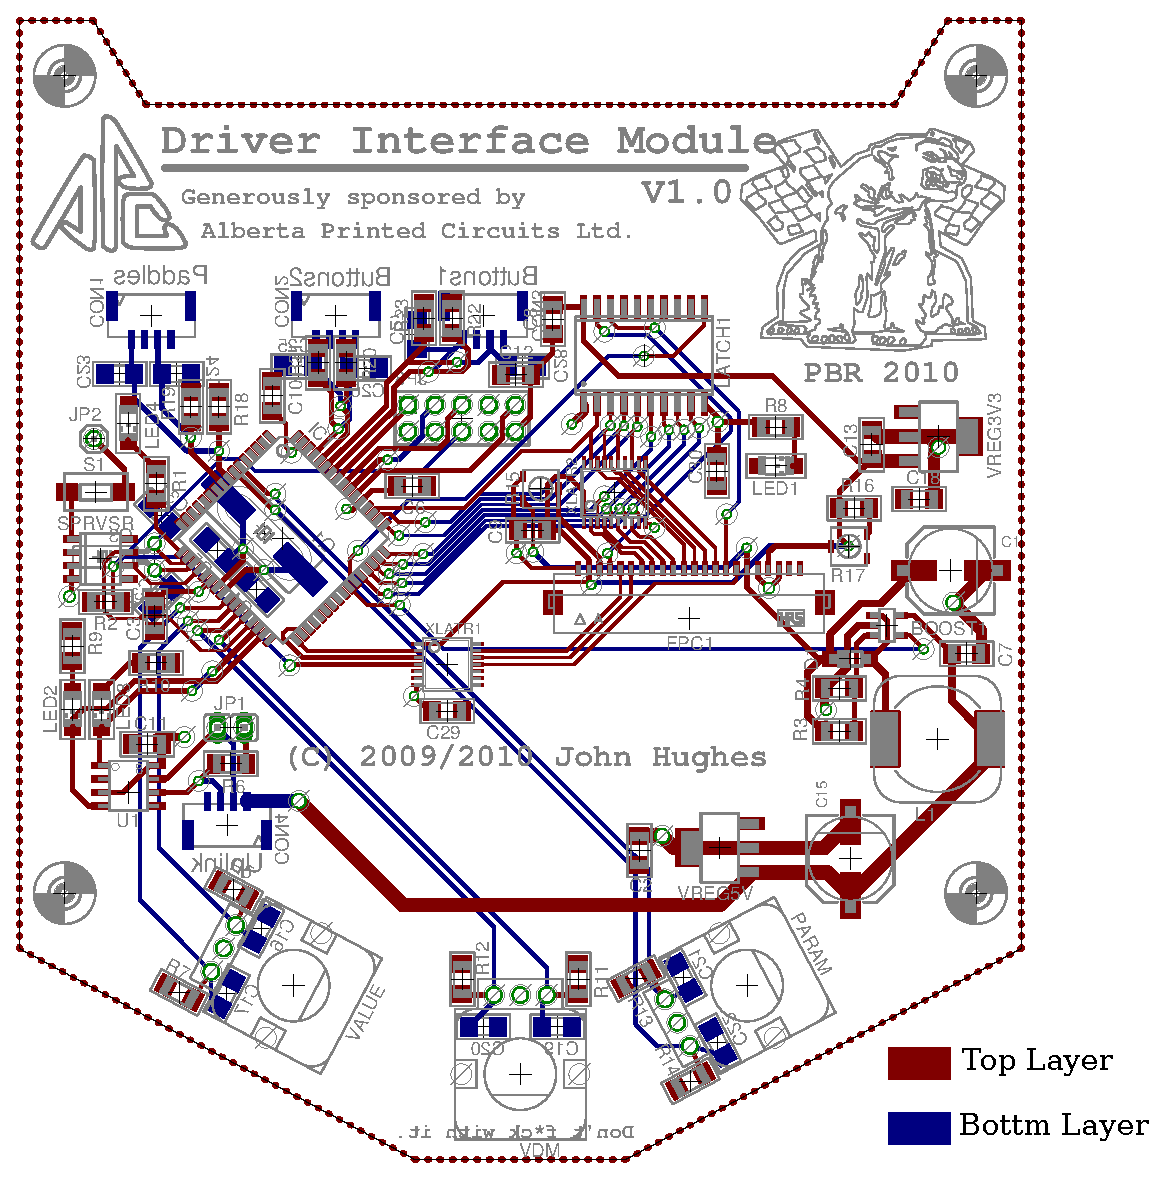
\includegraphics[width=3.5in,keepaspectratio]{implementation/figures/driver_interface_layout.eps}
  \caption{PCB Layout of the telemetry module.}
  \label{fig:driver_interface_layout}
\end{figure}

All four modules were populated with components and soldered by hand. Laser-cut mylar paste stencils were used to apply the solder. The process used to construct each module is as follows:

\begin{enumerate}
  \item Once the circuit boards had arrived from manufacture, simple electrical tests were made to validate the construction. Point-to-point checks of the ground and power planes were checked for continuity.
  \item An alcohol-based circuit board cleaner was applied to clean the surface of the boards.
  \item The mylar paste stencils were attached to the boards, and solder paste was applied using a syringe. The stencil was then removed.
  \item Individual components were placed on the pads with tweezers. The previously applied solder paste served as an adhesive.
  \item The board was placed into a toaster oven for approximately 7 minutes. 
\end{enumerate}

\begin{figure}[H]
 \centering
 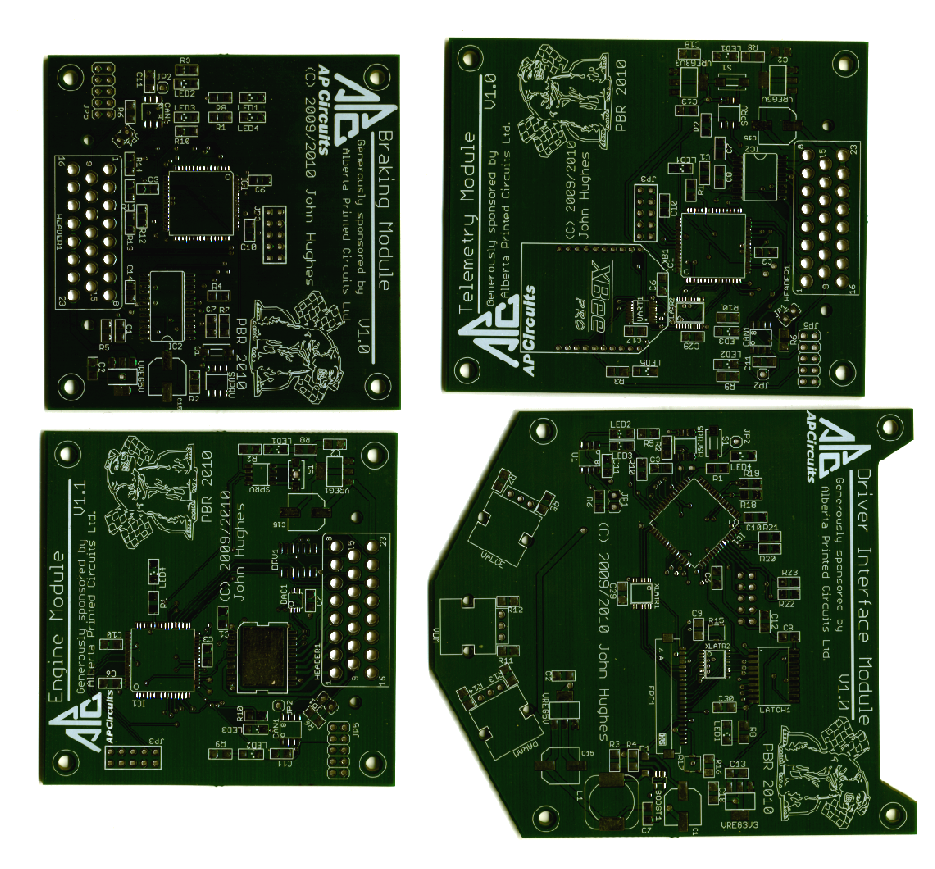
\includegraphics[width=4.25in,keepaspectratio]{implementation/figures/empty_pcbs.eps}
 \caption[Photographs of the bare circuit boards after manufacturing.]{Photographs of the bare circuit boards after manufacturing. Clockwise: Braking module, telemetry module, driver interface module, and engine and transmission module.}
 \label{fig:empty_pcbs}
\end{figure}

Two-minute warm up and cool-down periods were used before and after a 3 minute reflow phase. The warm-up period served to evaporate the solvents in the solder paste, while the gradual cool down was performed to avoid thermal shock.
